\documentclass[conference]{IEEEtran}
\IEEEoverridecommandlockouts
% The preceding line is only needed to identify funding in the first footnote. If that is unneeded, please comment it out.
\usepackage{cite}
\usepackage{amsmath,amssymb,amsfonts}
\usepackage{algorithmic}
\usepackage{graphicx}
\usepackage{textcomp}
\usepackage{hyperref}
\usepackage{xcolor}
\usepackage{booktabs}
\def\BibTeX{{\rm B\kern-.05em{\sc i\kern-.025em b}\kern-.08em
    T\kern-.1667em\lower.7ex\hbox{E}\kern-.125emX}}
\graphicspath{{Images/}{./}} 

\begin{document}

\title{Estimation of Vehicle Mass and Road Grade\\
{\footnotesize \large CS116.O11.KHCL - Machine Learning with Python: Final Project}
}

\author{\IEEEauthorblockN{Nguyen Hoang Tan} 
\IEEEauthorblockA{\textit{MSSV: 215214113} \\
21521413@gm.uit.edu.vn}
}

\maketitle

\begin{abstract}
    The Estimation of Vehicle Mass and Road Grade is a crucial aspect of modern transportation systems. This report introduces a machine learning-based approach to estimate both the mass of a vehicle and the grade of the road using relevant data.
\end{abstract}

\begin{IEEEkeywords}
    Machine Learning, Vehicle Mass Estimation, Road Grade Estimation, Sensor Data, Supervised Learning, Feature Engineering.
\end{IEEEkeywords}

\section{Introduction}
The Estimation of Vehicle Mass and Road Grade is a multifaceted challenge within the domain of transportation engineering, encompassing critical aspects such as fuel efficiency, vehicle performance, and overall safety. This project leverages machine learning methodologies to address this complex problem. We employ \href{https://scikit-learn.org/stable/modules/generated/sklearn.ensemble.RandomForestClassifier.html}{\textbf{Random Forest Classifier}} for Vehicle Mass and \href{https://scikit-learn.org/stable/modules/generated/sklearn.neighbors.KNeighborsRegressor.html}{\textbf{K-Nearest Neighbors Regressor}} for Road Grade estimation, focusing on the utilization of diverse signals collected from a vehicle to predict both its mass and the grade of the road it traverses.

\section{Dataset Description}
The dataset used in this project comprises eleven signals obtained from a vehicle, with the first nine serving as input features, and the last two as output variables. Notably, the data lacks time information, and the order of recordings has been deliberately scrambled. Each record in the dataset represents an individual frame, and the absence of temporal information necessitates an algorithmic approach that operates independently on each frame.

The signals include key parameters such as engine speed, vehicle speed, torque-related metrics, clutch and engine operation status, as well as the desired torque or torque limit. Of particular significance are the signals indicating road slope and the vehicle's mass, represented as either 38 t or 49 t.


\section{Exploratory Data Analysis (EDA)}
Before delving into the machine learning models, it is crucial to conduct an Exploratory Data Analysis (EDA) to gain insights into the dataset's characteristics and identify potential patterns or anomalies. 

\noindent \textbf{Data Integrity Check} \hspace{0.2em} Checking for missing values. Fortunately, the dataset demonstrates completeness, as no null values are present across any of the features.

\noindent \textbf{Outlier Detection} \hspace{0.2em} Generate box plots for each feature (excluding the target variable, Vehicle\_Mass) to identify potential outliers. 

\begin{figure}[h]
    \centering
    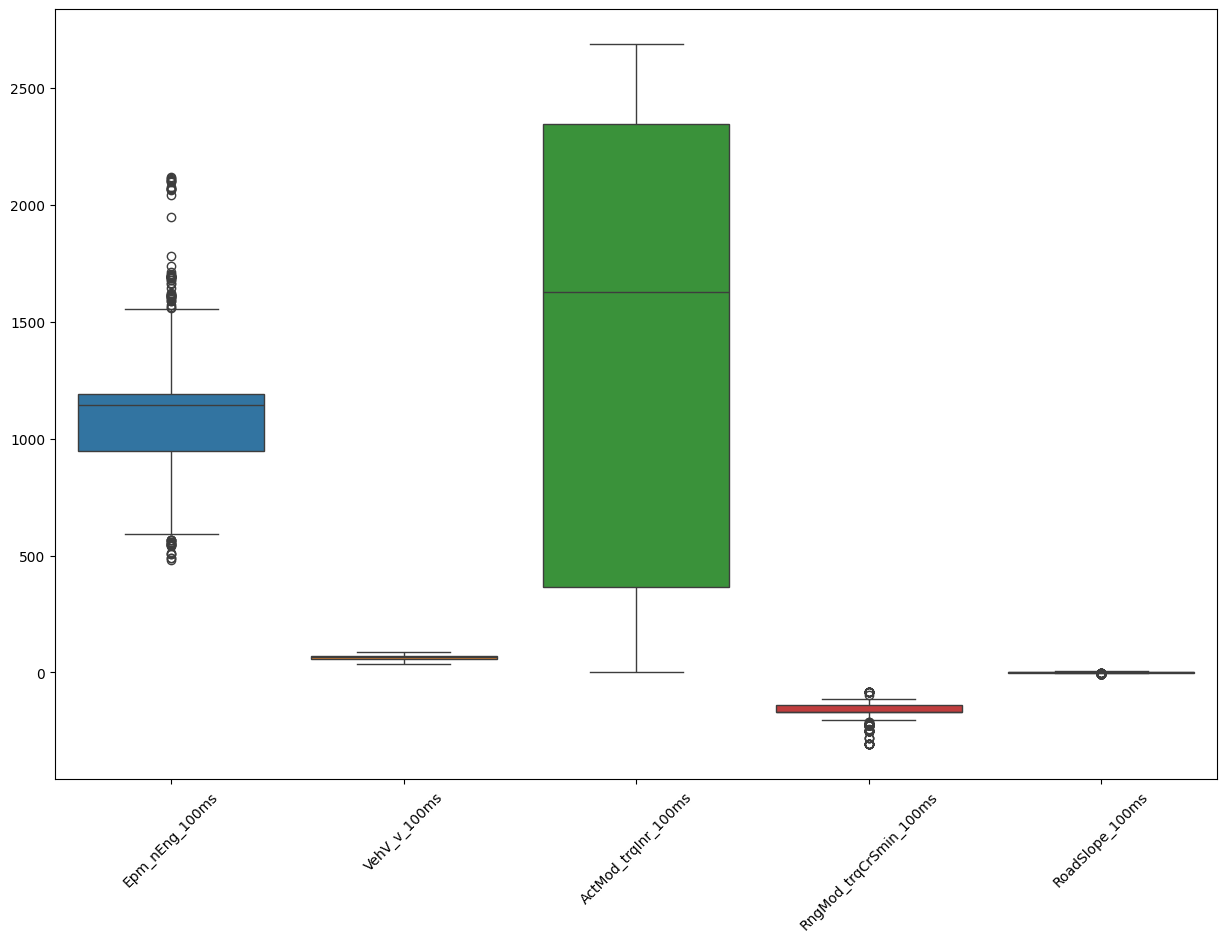
\includegraphics[width=0.5\textwidth]{Boxplot.png}
    \caption{Box Plot of Feature Columns }
    \label{boxplot}
\end{figure}

Figure \ref{boxplot} revealed the presence of numerous outliers across several features, potentially impacting the performance of machine learning models.

To mitigate the influence of outliers, We can utilize the \href{https://scikit-learn.org/stable/modules/generated/sklearn.preprocessing.RobustScaler.html}{\textbf{RobustScaler}} during the feature scaling process. \\

\noindent \textbf{Correlation Analysis} \hspace{0.2em} Table \ref{tab:correlation} provides insights into the relationships between variables, highlights correlations between features. Notably, `\textbf{RoadSlope\_100ms}` displays significant positive correlations with `\textbf{ActMod\_trqInr\_100ms}` and `\textbf{RngMod\_trqCrSmin\_100ms}`'.

\begin{table}[ht]
    \centering
    \begin{tabular}{lcc}
      \toprule
      & \textbf{RoadSlope\_100ms} & \textbf{Vehicle\_Mass} \\
      \midrule
      \textbf{RoadSlope\_100ms} & 1.000000 & 0.257673 \\
      \textbf{ActMod\_trqInr\_100ms} & 0.743515 & 0.084114 \\
      \textbf{RngMod\_trqCrSmin\_100ms} & 0.459027 & 0.604168 \\
      \textbf{Vehicle\_Mass} & 0.257673 & 1.000000 \\
      \textbf{Epm\_nEng\_100ms} & 0.138132 & 0.156700 \\
      \textbf{VehV\_v\_100ms} & -0.705378 & -0.630015 \\
      \bottomrule
    \end{tabular}
    \caption{Correlation Matrix of Features}
    \label{tab:correlation}
\end{table}

Additionally, the strong negative correlation $(-0.63)$ between `\textbf{VehV\_v\_100ms}` and `\textbf{RngMod\_trqCrSmin\_100ms}` suggests the possibility of creating a new combined feature for improving model performance.

\begin{figure*}[t]
    \centering
    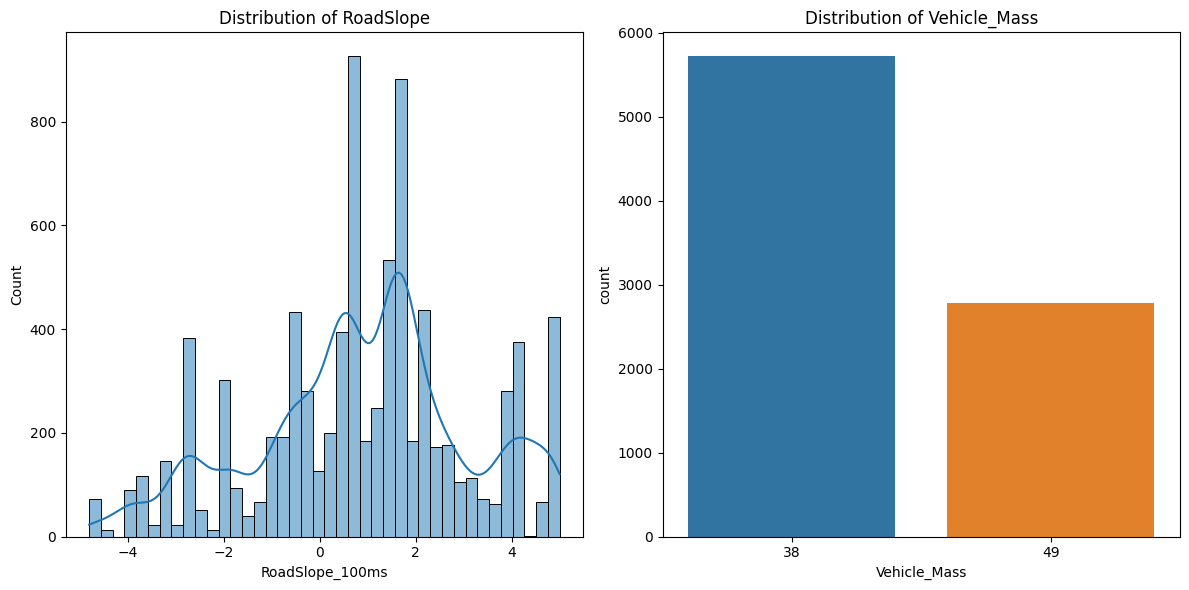
\includegraphics[width=\textwidth, height=0.3\textheight]{Distribution.png}
    \label{fig:roadslopedistribution}
\end{figure*}



\section{Data Preprocessing}
Having identified outliers, correlations, and distributions in the previous step, this section focuses on optimizing the dataset for the task. 
\subsection{Feature Engineering and Reformatting}
\begin{itemize}
\item Irrelevant constant features (`\textbf{CoVeh\_trqAcs\_100ms}`, `\textbf{Com\_rTSC1VRVCURtdrTq}`, `\textbf{Clth\_st`}, `\textbf{CoEng\_st}`, `\textbf{Com\_rTSC1VRRDTrqReq}`) are dropped as they provide no discriminatory information to distinguish between different instances. . 

\item The `\textbf{Vehicle\_Mass}`' column is reformatted to binary encoding for classification.


\end{itemize}

We create a new feature `\textbf{Combined\_VehV\_RngMod}` by combining '\textbf{RngMod\_trqCrSmin}' and '\textbf{VehV\_v}' using formula \ref{eq:1}. This combination is motivated by the strong negative correlation of $-0.63$ observed between these two variables.

\begin{equation} \label{eq:1}
    \hspace{-1em} Combined\_VehV\_RngMod = \dfrac{RngMod\_trqCrSmin\_100ms}{VehV\_v\_100ms}
\end{equation}

\subsection{Task-specific Dataset Splitting}
We initiate the dataset split into features and targets for both the regression and classification tasks, employing the same feature set for both predictions. 

However, we also introduce an alternative `\textbf{MultiTask}` approach. In this strategy, we utilize the predicted vehicle mass values to augment the prediction of road slope. \\

\noindent \textbf{Train-Dev-Test Splitting} \hspace{0.2em} The dataset is partitioned into training, development, and test sets for both regression and classification tasks. The distribution of the dataset across these sets is as follows:

\begin{itemize}
    \item Training Set: 70\%
    \item Development Set: 15\%
    \item Test Set: 15\%
\end{itemize}

\subsection{Feature Scaling}
As we observed numerous outliers in various features (Figure \ref{boxplot}). We address this problem by applying \href{https://scikit-learn.org/stable/modules/generated/sklearn.preprocessing.RobustScaler.html}{Robust scaling} to the features to ensure their uniformity across different scales. 

I also experimented with alternative scaling methods to assess their impact on the overall model performance. The evaluation results are presented in Table \ref{tab:model_performance}.

\begin{table}[h]
    \centering
    \caption{Model Performance with Different Scaling Methods}
    \begin{tabular}{lcc}
    \toprule
    \textbf{Scaling Method} & \textbf{Public Sets} & \textbf{Private Sets} \\
    \midrule
    RobustScaler & 98.86 & 75.5 \\
    StandardScaler & 84.46 & 68.52 \\
    MinMaxScaler & 81.2 & - \\
    MaxAbsScaler & 79.64 & - \\
    Normalizer & 64.73 & - \\
    PowerTransformer & 53.5 & - \\
    QuantileTransformer & 52.8 & - \\
    \bottomrule
    \end{tabular}
    \begin{flushleft}
        \small\textit{Note: Due to limited submit attempts for private sets, evaluation was performed with only two scalers.}
        \end{flushleft}
    \label{tab:model_performance}
    \end{table}
    
\section{Model Selection}
\subsection{Some Common Mistakes}\label{SCM}
\begin{itemize}
\item The word ``data'' is plural, not singular.
\item The subscript for the permeability of vacuum $\mu_{0}$, and other common scientific constants, is zero with subscript formatting, not a lowercase letter ``o''.
\item In American English, commas, semicolons, periods, question and exclamation marks are located within quotation marks only when a complete thought or name is cited, such as a title or full quotation. When quotation marks are used, instead of a bold or italic typeface, to highlight a word or phrase, punctuation should appear outside of the quotation marks. A parenthetical phrase or statement at the end of a sentence is punctuated outside of the closing parenthesis (like this). (A parenthetical sentence is punctuated within the parentheses.)
\item A graph within a graph is an ``inset'', not an ``insert''. The word alternatively is preferred to the word ``alternately'' (unless you really mean something that alternates).
\item Do not use the word ``essentially'' to mean ``approximately'' or ``effectively''.
\item In your paper title, if the words ``that uses'' can accurately replace the word ``using'', capitalize the ``u''; if not, keep using lower-cased.
\item Be aware of the different meanings of the homophones ``affect'' and ``effect'', ``complement'' and ``compliment'', ``discreet'' and ``discrete'', ``principal'' and ``principle''.
\item Do not confuse ``imply'' and ``infer''.
\item The prefix ``non'' is not a word; it should be joined to the word it modifies, usually without a hyphen.
\item There is no period after the ``et'' in the Latin abbreviation ``et al.''.
\item The abbreviation ``i.e.'' means ``that is'', and the abbreviation ``e.g.'' means ``for example''.
\end{itemize}
An excellent style manual for science writers is \cite{b7}.

\subsection{Authors and Affiliations}
\textbf{The class file is designed for, but not limited to, six authors.} A 
minimum of one author is required for all conference articles. Author names 
should be listed starting from left to right and then moving down to the 
next line. This is the author sequence that will be used in future citations 
and by indexing services. Names should not be listed in columns nor group by 
affiliation. Please keep your affiliations as succinct as possible (for 
example, do not differentiate among departments of the same organization).

\subsection{Identify the Headings}
Headings, or heads, are organizational devices that guide the reader through 
your paper. There are two types: component heads and text heads.

Component heads identify the different components of your paper and are not 
topically subordinate to each other. Examples include Acknowledgments and 
References and, for these, the correct style to use is ``Heading 5''. Use 
``figure caption'' for your Figure captions, and ``table head'' for your 
table title. Run-in heads, such as ``Abstract'', will require you to apply a 
style (in this case, italic) in addition to the style provided by the drop 
down menu to differentiate the head from the text.

Text heads organize the topics on a relational, hierarchical basis. For 
example, the paper title is the primary text head because all subsequent 
material relates and elaborates on this one topic. If there are two or more 
sub-topics, the next level head (uppercase Roman numerals) should be used 
and, conversely, if there are not at least two sub-topics, then no subheads 
should be introduced.

\subsection{Figures and Tables}
\paragraph{Positioning Figures and Tables} Place figures and tables at the top and 
bottom of columns. Avoid placing them in the middle of columns. Large 
figures and tables may span across both columns. Figure captions should be 
below the figures; table heads should appear above the tables. Insert 
figures and tables after they are cited in the text. Use the abbreviation 
``Fig.~\ref{fig}'', even at the beginning of a sentence.

\begin{table}[htbp]
\caption{Table Type Styles}
\begin{center}
\begin{tabular}{|c|c|c|c|}
\hline
\textbf{Table}&\multicolumn{3}{|c|}{\textbf{Table Column Head}} \\
\cline{2-4} 
\textbf{Head} & \textbf{\textit{Table column subhead}}& \textbf{\textit{Subhead}}& \textbf{\textit{Subhead}} \\
\hline
copy& More table copy$^{\mathrm{a}}$& &  \\
\hline
\multicolumn{4}{l}{$^{\mathrm{a}}$Sample of a Table footnote.}
\end{tabular}
\label{tab1}
\end{center}
\end{table}

\begin{figure}[htbp]
% \centerline{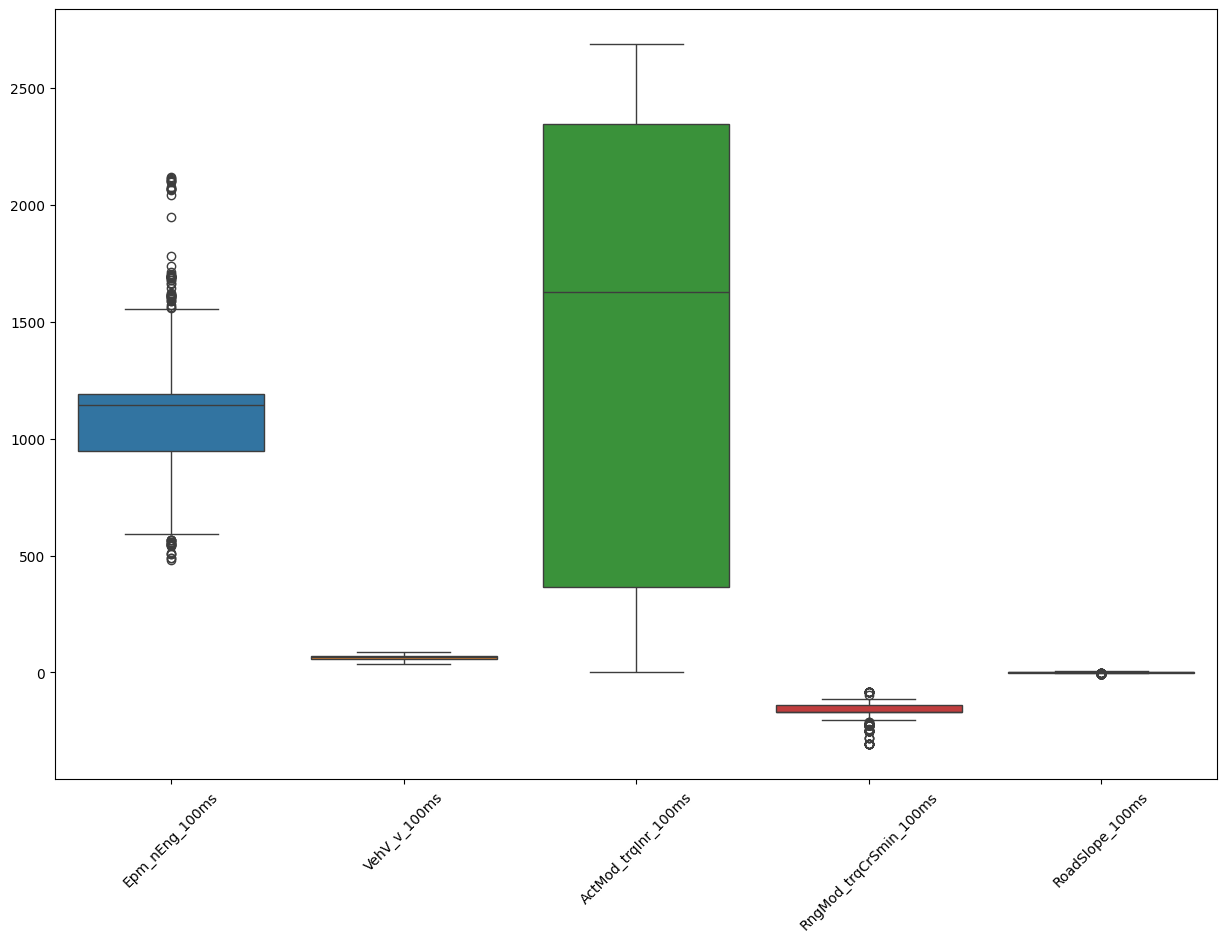
\includegraphics{Boxplot.png}}
\caption{Example of a figure caption.}
\label{fig}
\end{figure}

Figure Labels: Use 8 point Times New Roman for Figure labels. Use words 
rather than symbols or abbreviations when writing Figure axis labels to 
avoid confusing the reader. As an example, write the quantity 
``Magnetization'', or ``Magnetization, M'', not just ``M''. If including 
units in the label, present them within parentheses. Do not label axes only 
with units. In the example, write ``Magnetization (A/m)'' or ``Magnetization 
\{A[m(1)]\}'', not just ``A/m''. Do not label axes with a ratio of 
quantities and units. For example, write ``Temperature (K)'', not 
``Temperature/K''.

\section*{Acknowledgment}

The preferred spelling of the word ``acknowledgment'' in America is without 
an ``e'' after the ``g''. Avoid the stilted expression ``one of us (R. B. 
G.) thanks $\ldots$''. Instead, try ``R. B. G. thanks$\ldots$''. Put sponsor 
acknowledgments in the unnumbered footnote on the first page.

\section*{References}

Please number citations consecutively within brackets \cite{b1}. The 
sentence punctuation follows the bracket \cite{b2}. Refer simply to the reference 
number, as in \cite{b3}---do not use ``Ref. \cite{b3}'' or ``reference \cite{b3}'' except at 
the beginning of a sentence: ``Reference \cite{b3} was the first $\ldots$''

Number footnotes separately in superscripts. Place the actual footnote at 
the bottom of the column in which it was cited. Do not put footnotes in the 
abstract or reference list. Use letters for table footnotes.

Unless there are six authors or more give all authors' names; do not use 
``et al.''. Papers that have not been published, even if they have been 
submitted for publication, should be cited as ``unpublished'' \cite{b4}. Papers 
that have been accepted for publication should be cited as ``in press'' \cite{b5}. 
Capitalize only the first word in a paper title, except for proper nouns and 
element symbols.

For papers published in translation journals, please give the English 
citation first, followed by the original foreign-language citation \cite{b6}.

\begin{thebibliography}{00}
\bibitem{b1} G. Eason, B. Noble, and I. N. Sneddon, ``On certain integrals of Lipschitz-Hankel type involving products of Bessel functions,'' Phil. Trans. Roy. Soc. London, vol. A247, pp. 529--551, April 1955.
\bibitem{b2} J. Clerk Maxwell, A Treatise on Electricity and Magnetism, 3rd ed., vol. 2. Oxford: Clarendon, 1892, pp.68--73.
\bibitem{b3} I. S. Jacobs and C. P. Bean, ``Fine particles, thin films and exchange anisotropy,'' in Magnetism, vol. III, G. T. Rado and H. Suhl, Eds. New York: Academic, 1963, pp. 271--350.
\bibitem{b4} K. Elissa, ``Title of paper if known,'' unpublished.
\bibitem{b5} R. Nicole, ``Title of paper with only first word capitalized,'' J. Name Stand. Abbrev., in press.
\bibitem{b6} Y. Yorozu, M. Hirano, K. Oka, and Y. Tagawa, ``Electron spectroscopy studies on magneto-optical media and plastic substrate interface,'' IEEE Transl. J. Magn. Japan, vol. 2, pp. 740--741, August 1987 [Digests 9th Annual Conf. Magnetics Japan, p. 301, 1982].
\bibitem{b7} M. Young, The Technical Writer's Handbook. Mill Valley, CA: University Science, 1989.
\end{thebibliography}
\vspace{12pt}
\color{red}
IEEE conference templates contain guidance text for composing and formatting conference papers. Please ensure that all template text is removed from your conference paper prior to submission to the conference. Failure to remove the template text from your paper may result in your paper not being published.

\end{document}
